\documentclass[iop,apj]{emulateapj}
\pdfoutput=1 %for arxiv submission to use pdf
\usepackage{apjfonts}
\usepackage{natbib}
\usepackage{epstopdf}
\usepackage{gensymb}
\usepackage{longtable}
\usepackage{amsmath,amstext,textcomp}
\usepackage[breaklinks,colorlinks,citecolor=blue,linkcolor=magenta]{hyperref} 
\usepackage[all]{hypcap} %Links go to figures. This breaks deluxetables; use \capstartfalse \capstarttrue around deluxetables to fix it.
\renewcommand{\sectionautorefname}{\S} %for \autoref
\renewcommand{\subsectionautorefname}{\S} %for \autoref
\renewcommand{\subsubsectionautorefname}{\S} %for \autoref

\newcommand{\Reff}{R$_{\rm eff}$}
\newcommand{\Msun}{M$_{\odot}$}

%\renewcommand{\deg}{\ensuremath{^{\circ}}\xspace} %defines a degree symbol

\shorttitle{CCGs in the RESOLVE Survey}
\shortauthors{Snyder et al.}

\begin{document}

\title{Compact Core Galaxies in the RESOLVE Survey}
\author{Elaine M. Snyder\altaffilmark{1}}
\author{Sheila J. Kannappan\altaffilmark{1}}
\author{Dara J. Norman\altaffilmark{2}}
\author{Ashley S. Bittner\altaffilmark{1}}
\author{Mark A. Norris\altaffilmark{3}}
\author{Kathleen D. Eckert\altaffilmark{1}}
\author{Ian Dell'Antonio\altaffilmark{4}}
\author{Callie Hood\altaffilmark{1}}
\author{Samantha Dallas\altaffilmark{4}}
\author{David V. Stark\altaffilmark{1}}
\author{Amanda J. Moffett\altaffilmark{1,5}}
\author{the RESOLVE Team}
\affil{$^1$Department of Physics and Astronomy, University of North Carolina, 141 Chapman Hall CB 3255, Chapel Hill, NC 27599, USA; emsnyder@live.unc.edu}
\affil{$^2$National Optical Astronomical Observatory, 950 N Cherry Ave, Tucson, AZ 85719, USA}
\affil{$^3$Jeremiah Horrocks Institute, University of Central Lancashire, Preston, PR1 2HE, United Kingdom}
\affil{$^4$Department of Physics, Brown University, Box 1843, 182 Hope Street, Barus \& Holley, Providence, RI 02912} 
\affil{$^5$International Centre for Radio Astronomy Research (ICRAR), The University of Western Australia, 35 Stirling High-
way, Crawley, WA 6009, Australia}
\begin{abstract}
We analyze the complete set of 96 ``compact core galaxies'' (CCGs) in the volume-limited RESOLVE survey to investigate their formation and evolution in relation to compact galaxies such as ultra compact dwarfs (UCDs), compact ellipticals (cEs), and dwarf ellipticals (dEs) across a broad statistical distribution of environments. To identify CCGs, we use \textsc{Galfit} to perform one- and two-component S\'ersic fits for all galaxies in RESOLVE with UKIDSS $Y$-band imaging (98\% of the survey), which produces seeing-deconvolved effective radius (\Reff) measurements. The one component fits are used to select candidate CCGs with \Reff\ $< 1000$ pc, and we then perform new two component fits to these galaxies with the S\'ersic n of the second component held fixed at 1 for an exponential disk. We finalize the CCG sample by selecting on core-only (first component) \Reff\ $<800$pc, an upper limit that encompasses all of the similarly compact stellar systems (UCDs, cEs) included in the Archive of Intermediate Mass Stellar Systems (AIMSS) catalog. We quantify the amount of light in the core and envelope of each CCG by taking the logarithm of the ratio of the light in each component. The result is a smooth continuum of CCGs that range from envelope-dominated to core+envelope to core-dominated. With GALEX $NUV$, SDSS $ugriz$, and 2MASS/UKIDSS $YJHK$ data, we derive colors and star formation histories and find that a significant number of CCGs live on the blue sequence and have recently formed stars. We find that CCGs naturally occur in a range of environments from free floating to cluster. We also derive velocity dispersions ($\sigma$) for 8 CCGs from Gemini IFU data and SOAR spectroscopy. Comparing to other RESOLVE galaxies and AIMSS cEs/dEs, we search for CCGs offset to higher or lower dispersion in the dispersion-stellar mass relation, which may indicate tidal stripping (as expected for cEs) or dissipative formation (as expected for dEs), respectively. Initial results show 4 CCGs likely following the dissipative formation track and 4 CCGs that are intermediate.

\end{abstract}

\keywords{galaxies: formation, evolution --- surveys}
\maketitle

%%%%%%%%%%%%%%%%%%%%%%%%%%%%%%%
%%%%%%%%%%%%%%%%%%%%%%%%%%%%%%%
\section{Introduction}
\label{intro}

  The term compact stellar system (CSS) encompasses a class of galaxies that spans the radius range between globular clusters (GCs) and normal elliptical galaxies (Es). Different types of CSSs include compact elliptical galaxies \citep[cEs;][]{Faber1973} and ultra compact dwarf galaxies \citep[UCDs;][]{Phillipps2001}. There are many unanswered questions about how CSSs form and evolve through time. One fact that makes the study of these compact galaxies so intriguing is their apparent scarcity, which raises the question as to whether they are an intermediate and short-lived evolutionary phase in the life of a galaxy, or simply hard to find due to their size. Only in the last 15 years have we discovered enough ($\sim 40$) of these objects to enable studies of their formation scenarios.

CSSs have half-light radii (\Reff) ranging typically from $\sim$10--600 pc \citep[e.g.,][]{Norris2014}, and there are multiple ideas for how they form. The smaller of the CSSs, UCDs may simply be the high mass extension of the GC population \citep{Drinkwater2000, Mieske2002}. The is also evidence that UCDs are created via the tidal stripping of nucleated dwarf galaxies \citep{Bekki2001, Bekki2003, Norris2011, Jennings2015, Zhang2015}. \citet{Seth2014} find a supermassive black hole at the center of another UCD, providing further evidence of tidal stripping being common for UCDs. Similarly, cEs are thought to be the result of tidal stripping events, as argued for the prototypical cE, M32 \citep{Choi2002, Graham2002, Huxor2011}. More evidence is provided by the discovery of tidal streams near cEs \citep{SmithCastelli2008a,Chilingarian2009} and one cE, studied in \citet{Kormendy1997}, that is believed to host a central massive black hole. On the other hand, \citet{Wirth1984}, \citet{Kormendy2009}, and \citet{Kormendy2012a} argue that cEs are the low mass extension to the normal E population created via dissipative formation in gas rich environments, such as during mergers or in the two-phase formation process detailed in \citet{Oser2010}. One of the most successful recent searches for CSSs is the AIMSS catalog \citep{Norris2014}: with many newly discovered UCDs and cEs to examine, the authors argue that all of the above scenarios for UCD and cE formation occur.

In contrast to CSSs, dwarf elliptical galaxies \citep[dEs;][]{Sandage1985} and their nucleated counterparts \citep[dE,Ns;][]{Binggeli1984} are quite common, especially in clusters where they were first discovered. In fact, \citet{Binggeli1991} find that of 225 galaxies present in the center of Virgo cluster, 174 are classified as dEs or dE,Ns based on their surface brightness profiles. While dEs are typically larger than CSSs with \Reff\ ranging from $\sim600$~pc up to $\sim2000$~pc \citep[e.g.,][]{Norris2014}, the cores of dE,Ns can reach down to CSS-like sizes and reside within larger envelopes that are dE-sized. Similar to cEs, dEs are often thought to be either tidally stripped remnants \citep{Crnojevic2014} or the low mass extension to elliptical galaxies \citep{Kormendy2012a}. They could also be the remnants of late-type disk galaxies or luminous blue compact dwarfs that have been ram-pressure stripped and quenched as they enter the cluster environment \citep{Lisker2013, Crawford2016a}. There is also evidence that dE,Ns become UCDs as they fall deeper into the cluster core and are further stripped \citep{Pfeffer2013,Zhang2015,Liu2015}.

Given the similarities in formation scenarios between CSSs and dEs, we introduce the term ``compact core galaxy'' or ``CCG'' to encompass CSSs and dEs with core \Reff\ up to 800~pc. The goal of this paper is to study these galaxies as part of a continuum of compact galaxies in order to differentiate between formation scenarios. Clues to how CCGs form may be given by their environments,  morphology i.e., one- or two-component structure, star formation histories, and kinematics. We highlight these data below.

%environments
\textit{Environments.} CSSs have been found in a large range of environments thus far. UCDs were first discovered in the Fornax cluster \citep{Hilker1999, Drinkwater2000} and have since been found in the cores of several other clusters \citep{Price2009,Madrid2010,Jones2006,Mieske2009,Misgeld2008}, in groups \citep{Evstigneeva2007}, and near field galaxies \citep{Hau2009,Norris2011}. M32 was first discovered in our Local Group \citep{Faber1973} near M31, and more cEs have later been found in clusters \citep{Chilingarian2007,SmithCastelli2012,Price2009} and other groups \citep{Huxor2011,Chilingarian2010}. As stated previously, dEs and dE,Ns are common in clusters \citep{SmithCastelli2012,Koo1994,Guzman1996,Crawford2016a}, but have also been found near groups \citep{Crnojevic2014,Penny2014}. Only cEs have been found ``free floating'', meaning there is no host galaxy at all: \citet{Huxor2013} and \citet{Paudel2014} both find one cE separated from other galaxies by $\sim~840$ and $\sim~600$~kpc, respectively. 

Environment bears on formation scenarios in different ways. One possibility is that CSSs found in group or cluster environments may be tidally stripped remnants, whereas free floating CSSs may rather be dissipatively formed like Es. However, \citet{Chilingarian2015} argue that these free-floating cEs could actually be tidally-stripped cores that are ejected from groups and clusters during the tidal stripping process. The recent discovery of a free-floating GC and UCD that have likely been tidally stripped in \citet{Sandoval2015} supports this idea.

%structure
\textit{Morphologies.} CSSs have been found to exhibit either one component (i.e., just a core) or two component (i.e., a core plus a surrounding envelope of gas and stars) morphology. \citet{Graham2002} have shown that M32's light profile is best fit with a core plus a surrounding exponential disk profile, which they argue points toward a tidal-stripping origin. \citet{Pfeffer2013} use N-body simulations to predict that UCDs that are tidally stripped remnants will also display multi-component surface brightness profiles due to lingering outer galaxy structures. Conversely, dissipative processes such as the two-phase formation scenario proposed by \citet{Oser2010} cause cores to form as gas rushes to the center during mergers or the convergence of streams of cold gas and star formation begins. This core is then ``puffed up'' through time as it interacts with other galaxies. The free-floating cE discovered in \citet{Huxor2013}, shown to have only a one-component light profile, may be an example of the first step in this two-phase formation. It's important to note that these effects may vary based on the degree of stripping and how much time has passed since the stripping or dissipative formation occurred.

By their nomenclature, dEs and dE,Ns have already been divided into one and two component morphologies. Studies have found that dE,Ns are usually more common than dEs: \citet{Grant2005} find that the majority of Virgo cluster dwarfs are indeed nucleated and speculate that at least some of the nuclei were formed out of an existing non-nucleated galaxy from infalling gas. Another possibility is that the morphology is already in place as dEs/dE,Ns form: \citet{Mastropietro2005a} use N-body simulations to show that as the progenitors of dEs/dE,Ns enter clusters, their morphologies are greatly disrupted but disks may not be completely destroyed by ram pressure or tidal stripping, leaving the dEs/dE,Ns we observe today.

%colors
\textit{Star formation histories.} 
Colors and star formation rates are useful since they may point to recent star formation as a part of tidal stripping or dissipative formation. The typical thought is that CSSs are ``red and dead'', and some studies even cut on color when selecting CSS samples \citep{Chilingarian2015}. \citet{Drinkwater2000} have examined the stellar populations of CSSs and find that CSSs are usually best fit as having older stellar populations. However, \citet{Norris2011} find a UCD with young stellar populations and smoking gun signs of tidal stripping origins, including counter-rotating gas and a short dynamical friction timescale. \citet{Maraston2004} also find a young tidally formed UCD near the merger remnant galaxy NGC~7252. This evidence makes it clear that CCSs can have young and old stellar populations.

For dEs and dE,Ns, there is similar diversity in colors. \citet{SmithCastelli2012} find dEs in the Antlia cluster with both red and blue colors. \citet{Drinkwater2000} and \citet{Ferrarese2006} study the colors of dE,Ns and find that the cores of dE,Ns tend to have younger stellar populations compared to their host galaxies. \cite{Grant2005} also find that two-fifths of the Virgo dE,Ns have young cores compared to their envelopes, while three-fifths display the opposite trend. 

%kinematics
\textit{Kinematics.}  The last useful tool we have for discerning between formation scenarios is the galaxy's stellar velocity dispersion ($\sigma$). \citet{Bender1992} and \citet{Bekki2003} show that $\sigma$ will remain largely unchanged when tidal stripping occurs, even though the \Reff\ and stellar mass will be greatly reduced. Thus, galaxies that are offset to higher $\sigma$ in a Faber-Jackson (stellar mass -- $\sigma$) relation \citep{faber1976} are most likely tidally stripped, while galaxies falling along the relation are most likely the low-mass extension of normal Es. Lending evidence to this idea are the tidally-stripped UCD found in \citet{Maraston2004} and the prototypical cE, M32, both of which have much larger velocity dispersions than expected for their mass.

In this paper, we present a complete sample of CCGs derived from the volume-limited RESOLVE survey, along with key data quantifying their morphologies, environments, star formation histories, and kinematics. We use this sample to examine the formation scenarios and evolution of CSSs and dEs/dE,Ns simultaneously as a spectrum of compact galaxies that span the gap from GCs to Es. Because we have derived a complete sample from RESOLVE, our sample contains CCGs at every evolutionary stage. This paper is organized as follows. We describe our parent sample, the RESOLVE survey, in \autoref{resolve} and our comparison sample, the AIMSS catalog, in \autoref{aimss}. Our methods for performing seeing-deconvolved one and two component fits for the entire RESOLVE sample using \textsc{Galfit} are presented in \autoref{deconv}. We detail the selection of the CCG sample from the RESOLVE survey and quantify our CCG demographics in \autoref{CCGs}. We describe our photometric, environmental, and spectroscopic data and analysis in \autoref{methods}. We present a statistical distribution of environments, star formation histories, and velocity dispersions for the complete sample in \autoref{results}. In \autoref{discussion}, we present a discussion of our results in the context of CCG formation and evolution. Lastly, the summary and future work are given in \autoref{conclusions}.

%%%%%%%%%%%%%%%%%%%%%%%%%%%%%%%
%%%%%%%%%%%%%%%%%%%%%%%%%%%%%%%
\section{Samples}
\label{samples}

\subsection{The RESOLVE survey}
\label{resolve}

  We use the RESOLVE survey \citep[][Kannappan et al., in prep]{Kannappan2008} as the parent sample for our census of CCGs. RESOLVE is ideal because it is an unusually complete and volume-limited survey, which allows us to find CCGs at all evolutionary stages. RESOLVE falls within the footprint of the Sloan Digital Sky Survey \citep[SDSS,][]{York2000}, and covers equatorial strips in both semesters: A for the northern spring sky and B for the northern fall sky, which overlaps much of Stripe-82. With $\text{H}_{\circ} = 70~\text{km~s}^{-1}$, RESOLVE-A spans $\sim38,400~\text{Mpc}^3$ and occupies the region $131.25\degree~<~\text{RA}~<~236.25\degree$ and $0\degree~<~\text{Dec}~<~5\degree$, while RESOLVE-B spans $\sim13,700~\text{Mpc}^3$ and occupies the region $330\degree~<~\text{RA}~<~45\degree$ and $-1.25\degree~<~\text{Dec}~<~1.25\degree$. Both semesters cover the redshift range 4500 km s$^{-1} <$ cz $< 7000$ km s$^{-1}$.

RESOLVE's exceptional completeness is obtained by making use of multiple redshift surveys to recover galaxies that were missed in SDSS due to (i) fiber collisions, (ii) the ``shredding'' of galaxies in which the pipeline breaks up a single galaxy into individual pieces so no one piece meets the magnitude cut, and (iii) the intentional exclusion of low surface brightness galaxies ($\mu_{50} < 24.5$ mag arcsec$^{-2}$), even if they meet the magnitude cut. We supplement the SDSS main redshift survey with additional redshifts from archival sources, including the Updated Zwicky Catalog \citep{Falco1999}, HyperLeda \citep{Paturel2003}, 6dF \citep{Jones2009}, 2dF \citep{Colless2001}, GAMA \citep{Driver2011}, and ALFALFA \citep{Haynes2011}, to achieve $\sim12\%$ higher completeness in RESOLVE-A and $\sim25\%$ higher completeness in RESOLVE-B \citep{Eckert2015}.

With its improved redshift recovery, RESOLVE is complete down to absolute $r$-band magnitudes of $-17.33$ and $-17.0$ for the A and B semesters, respectively. To derive the stellar mass completeness limits of RESOLVE, \citet{Eckert2016} use the known stellar masses and magnitudes of all RESOLVE galaxies to determine the stellar mass limit above which no more than 2\% of objects have an $r$-band magnitude fainter than the stated magnitude completeness limit. These values are M$_{\star}~\sim~10^{8.9}$~\Msun~for the A semester and M$_{\star}~\sim~10^{8.7}$~\Msun~in the B semester \citep[Figure 8 in ][]{Eckert2016}. These stellar mass completeness limits allow us to reach down to CSSs with sizes and masses similar to cEs (see \autoref{morph} for more details), but restricts us from reaching down to UCD masses.

An important caveat to RESOLVE's completeness is that the survey is preferentially incomplete for the very objects this study is focused on, cEs. Such round objects can often be mistaken for stars in redshift surveys using tools such as the \texttt{class\_star} parameter in Source Extractor \citep{Bertin1996}. We are engaged in ongoing efforts to use photo-z estimates to recover some of these objects.

\subsection{The AIMSS catalog}
\label{aimss}

  We use the Archive of Intermediate Mass Stellar Systems (AIMSS) catalog \citep{Norris2014,Forbes2014,Janz2015} as a reference sample for our CCGs.  AIMSS is a catalog of spectroscopically confirmed CSSs found near field galaxies and in groups and clusters, and includes both previously known and newly discovered objects. The AIMSS CSS discovery process was as follows. First, a search was conducted in the HyperLeda redshift catalog \citep{Paturel2003} for all galaxies with M$_{\rm B}~<~-15$ and distances between $\sim 7$ and 200 Mpc (close enough to ensure any CSSs with \Reff\ $> 50$ pc would be resolved in any available HST imaging). The team then searched the Hubble Space Telescope archive for WFCP2, ACS, and WFC3 imaging within 150 kpc in projection of the selected galaxies. Next, Source Extractor was run on the HST images, and candidates were identified using a training set of previously known CSSs from the literature. After vetting by eye and cross-matching to ensure none are previously known, spectra were obtained for redshift confirmation and measurements of velocity dispersions. AIMSS also includes literature data for previously known UCDs, cEs, dEs, dE,Ns, dwarf spheroidals, dwarf S0s, young massive clusters, and Es. The catalog provides a compilation of absolute $V$-band magnitude, stellar mass, half-light radius, and velocity dispersion for each of its objects. Thus, though not a statistically-defined sample, AIMSS provides a useful reference catalog to which we can compare our CCGs. We also note that the objects in AIMSS are not decomposed, meaning their \Reff\ are all single component fits. We discuss this more in \autoref{discussion}.

\begin{figure*}[b]
\begin{center}
\includegraphics[scale=0.5]{galfitexample.eps}
\caption{Model inputs and outputs from \textsc{Galfit}. The left column shows the UKIDSS $Y$-band image cutout around the galaxy. The middle column shows the best fit \textsc{Galfit} model, and the right column shows the residuals (data-model). The top row shows the one component fit for one of the RESOLVE galaxies, rf0055. As seen in the residual image, the model is overfitting the inner bulge, and underfitting the outer envelope. The bottom row shows the two component fit for the same galaxy. We are now  able to fit both the inner bulge and the outer envelope. The residual is much cleaner, although there may be some spiral structure remaining.}
\label{fig:galfit}
\end{center}
\end{figure*}

\subsection{CCG sample selection}

\subsubsection{Deconvolution of RESOLVE galaxies}
\label{deconv}

  We begin our analysis by deriving seeing-deconvolved \Reff\ measurements for all galaxies in the RESOLVE sample. For this task we employ \textsc{Galfit} \citep{Peng2002} to deconvolve the seeing point spread function (PSF) and to perform one and two component fits to each galaxy. Deconvolution is especially important since the smallest galaxies in RESOLVE are most affected by seeing, and accurate radius measurements are crucial for the study of these objects. 

\textsc{Galfit} needs the following input files to function properly: an initial input file, an image of the galaxy, a PSF image, an image mask, and a constraint file. We obtain or construct these items as follows:

\begin{description}

\item[The initial input file]{The initial input file gives \textsc{Galfit} the file paths to the image, PSF, mask, and constraint file, and also holds the initial guesses for our fit parameters. For the one component fits, we set up our input file to include a section to measure the level of the sky background and another section to fit a S\'ersic profile \citep{Sersic1963, Sersic1968} to the galaxy. The S\'ersic model will find a best fit for the following parameters: central x \& y position of the model, integrated magnitude, \Reff, S\'ersic n, axial ratio (b/a), and position angle. These initial values for these parameters can just be rough guesses, but for our purposes, we use values for the magnitude, \Reff, b/a, and PA that are derived from RESOLVE's custom processed photometric data (see \autoref{phot} for more details).}

\item[Imaging data]{We use publicly-available high resolution $Y$-band imaging from the UKIDSS Large Area Survey \citep{Lawrence2007}. This data set was chosen because it covers both RESOLVE-A and RESOLVE-B and offers $\sim0.8''$ seeing resolution corresponding to $\sim350$pc at RESOLVE distances in turn letting us span down to the sizes of cE-like galaxies. The $Y$ band is advantageous too, since it probes the underlying stellar population and will not skew our measurements to larger radii if the galaxy is currently experiencing a starburst. We download $\sim10'\times10'$ images of each galaxy from the WFCAM Science Archive\footnote{\url{was.roe.ac.uk//}}}. While \textsc{Galfit} does not require images this large to operate normally, we choose this size so that there will be more stars in the field of view which is useful when constructing the PSF image. There are only 25 galaxies in RESOLVE (2\% of the survey) that do not have UKIDSS imaging and thus are excluded from our analysis.

\item[The PSF image]{\textsc{Galfit} uses the PSF image to deconvolve the galaxy light profile from the seeing, thereby removing the effects of atmospheric scattering of the galaxy light as the data was taken. We build our PSF image via the following steps.
\begin{enumerate}

\item We begin by running Source Extractor on the image to identify every object in the frame, including stars, galaxies, and even sometimes hot pixels. Source Extractor outputs a text file that has estimates of each object's flux, elongation, ellipticity, radius, and \texttt{class\_star}.

\item With this information, we select stars to use for building our PSF. The limiting parameters are (1) that the flux must be between $5,000-100,000$ counts to ensure no extremely faint or saturated stars are included, (2) that the ellipticity be less than 0.2 to ensure we are selecting round objects, (3) that the effective radius of the star be greater than 1 pixel to avoid selecting hot pixels, and (4) that \texttt{class\_star} is greater than 0.6 to ensure the objects we're picking are most likely stars. We also make sure the stars are not near the image edges, since there can sometimes be image artifacts there. Lastly, we make sure to not include the galaxy we are going to fit, since the cE-like galaxies can sometimes appear to be stars.

\item We next make $101\times101$ pixel cutouts of each object detected, with the flux peak at pixel $x=51,y=51$. 

\item Background subtraction is then performed by taking the median of the entire cutout and then subtracting each pixel by this median value.

\item We then reject any of the cutouts that have a background median value greater than $2\sigma$ from the mean of the background median values for every cutout. This ensures we are not including any cutouts that have stars with large or bright neighboring objects. We are now left with background-subtracted cutouts of stars with no neighbors that could affect our stacking. 

\item Before we can combine all the cutouts, we must normalize the flux of each central star to the same amplitude. To do this, we run each cutout through Source Extractor once more to obtain the fluxes of each central star and use these to weight the cutouts accordingly. We calculate the weight for each cutout as follows: (1) we find the central star with the highest flux of all the cutouts and then (2) divide every flux by this maximum flux. We then divide each cutout by its corresponding weight, which makes each central star have the same amplitude.

\item We then take the median of all the weighted cutouts to create a semi-complete PSF.

\item Lastly, we normalize the semi-complete PSF from Step 7 by dividing each pixel in the frame by the total flux in the image. We find the total image flux by taking the mean of each pixel and multiplying that by the number of pixels in the image (so, $101\times101$). This ensures that the final PSF image is normalized, i.e., the sum of the flux in each pixel of the cutout would equal one.    

\end{enumerate}

Our last step is to fit a 2D Gaussian to the PSF to determine a rough estimate seeing full width half max (FWHM), as a sanity check. We find that the average FWHM for all PSFs is $\sim 0.9''$, only slightly worse than the $\sim 0.8''$ seeing expected for UKIDSS imaging.}

\item[The mask image]{\textsc{Galfit} uses the mask image to ignore any objects neighboring our galaxy while it is completing the fit.The first step in making the mask is to create an image that has the same dimensions as our input image but with each pixel value equaling zero. We again use Source Extractor to compile a list of all the objects in the input image, and  use this list to replace the pixel values at the coordinates of the located objects with one.}

\item[The constant file]{The constraint file hosts the limits we are willing to accept for each of the fit parameters. The constraints for x \& y position in the image, integrated magnitude, \Reff, S\'ersic n, axial ratio (b/a), and position angle for the one component fits are listed in \autoref{constrtable}. We change the constraint file for the two component fits later in the analysis.}

\end{description}

\begin{table}[htdp]
\begin{center}
\begin{tabular}{cc} \hline
parameter & constraint  \\ \hline
x \& y position & $\pm5$ pixels from input value \\
integrated magnitude & 0 -- 40 \\ 
\Reff\ & 0.2 -- 750 pixels \\ 
S\'ersic n & 0.1 -- 8 \\ 
axial ratio (b/a) & 0 -- 1 \\
position angle (PA) & -360 -- 360 \\ \hline
\end{tabular}
\end{center}
\caption{Summary of the constraints imposed on our \textsc{Galfit} models for our initial one component fits for the entire RESOLVE sample.}
\label{constrtable}
\end{table}%

  We use all of the above to obtain a one component, seeing-deconvolved fit for every galaxy in the RESOLVE survey. We then perform the two component fits as follows. We use the output of the one component fit as the basis of the input file for the two component fit. The first two sections in the two component fit initial input file will be identical to the output of the one component fit (except that the names of the files to be output are changed). We then add a third section to include a second S\'ersic fit, and change the initial guess for \Reff\ to be double that of the one component best fit. This gives \textsc{Galfit} an idea to fit on both a core and envelope. The PSF, image, and mask image will all be the same as before. We add to the constraint file the same constraints as listed in \autoref{constrtable}, but for the third section. In other words, there will be two sets of constraints in the file now, with the first set applying to the first S\'ersic fit and the second set applying the second S\'ersic fit. The constraints for each parameter are the same for both sets. We do not further constrain the two component fits since we are looking for general fits to the wide variety of galaxies in RESOLVE and do not want to over-constrain the fits.

For both the one and two component fits, \textsc{Galfit} outputs a text file with the best fits for central x \& y position of the model, integrated magnitude, \Reff, S\'ersic n, axial ratio (b/a), and position angle as well as the $\chi^2$, $\chi^2/\nu$ and number of degrees of freedom for the fit. Also output is a fits file that contains the data, best fit model, and residual images. See \autoref{fig:galfit} for example one and two component fits for the RESOLVE galaxy rf0055.

\subsubsection{Selection of CCGs}
\label{CCGs}

\begin{figure*}[hbpt!]
\begin{center}
\includegraphics[scale=0.65]{coretoenvelopeims.eps}
\caption{Five of the 96 CCGs in the final sample arranged in order from envelope-only to core+envelope to core-only. Images are taken from the SDSS-DR8 image list tool. The galaxy rf0250 is an example of one of eleven CCGs that was fit with a large diffuse envelope and has hence been reclassified as ``core-dominated''.}
\label{fig:pics}
\end{center}
\end{figure*}

Now that we have seeing-deconvolved \Reff\ values for the entire RESOLVE sample, we begin our search for compact core galaxies. We select a maximum cutoff core-only radius for CCGs at 800~pc. Comparing to the CSSs and dEs/dE,Ns in the AIMSS catalog, this upper limit ensures that we are selecting CSSs in RESOLVE with \Reff\ up to 600~pc and lets us include the smallest dEs and dE,Ns as well.

We start our search for CCGs by using the one component fit from the above analysis and select galaxies with \Reff\ values $<1000$~pc. Since we are looking for galaxies with compact cores, extending to \Reff\ $\sim 1000$~pc allows us to select objects with cores that are dominating the light and therefore may have a smaller core \Reff\ in a two component fit. We do note that this limit is arbitrary, and will be relaxed in the future to allow CCGs with larger envelopes be included in the sample (see \autoref{conclusions}). We also limit the  $\chi^2/\nu$ to be $<1.3$, since values above this represent galaxies with large residuals left over, which are normally spiral or irregular galaxies. After this selection, we are left with 124 galaxies in the CCG candidate sample.

Next, we perform new two component fits using different fitting constraints: (1) the central x and y positions are taken from the one component fit and are held constant for both S\'ersic components, (2) the \Reff\ of the second S\'ersic component fit is constrained to always be larger than that of the first S\'ersic component fit, and (3) the S\'ersic n of the second component is held constant at 1 representing an exponentially decreasing disk profile. We let the values of \Reff, integrated magnitude, b/a ratio, and PA change for both fits. By doing this, we are forcing \textsc{Galfit} to fit on a core (the first S\'ersic component fit) and disky envelope (the second S\'ersic component fit) for each CCG candidate.

We then examine the fits by eye and create our final CCG sample by selecting where the core \Reff\ $< 800$ pc and $\chi^2/\nu < 1.3$ to again exclude poor fits. Our sample is thus comprised of 96 CCGs in total (63 from RESOLVE-A and 33 from RESOLVE-B). This represents $\sim6$\% of the total RESOLVE galaxy sample. \autoref{fig:radius} shows their distribution in stellar mass and decomposed \Reff\ compared to other RESOLVE galaxies and the AIMSS cEs and dEs. For the RESOLVE sample, we are plotting the one component fits, while for the CCGs, we are plotting the core \Reff\ from the fixed two component fits. 

We quantify the amount of light in the core vs.~the envelope by taking a ratio of the flux in each component. We compute the fluxes using $m = -2.5 \times \log({\rm flux})$, where $m$ is the integrated magnitude output from \textsc{Galfit}. We note that \textsc{Galfit} calculates the integrated magnitude for S\'ersic profiles using the equations:

\begin{eqnarray}
\text{flux}~&=&~2~\text{R}_{eff}^2~\Sigma_e~\text{e}^{\kappa}~n~(\kappa)^{-2n}~\Gamma(2n)~(b/a)~/~R(C_0; m) \\
\kappa~&\approx&~1.999~n~-~0.327\\
m~&=&~-2.5~\log_{10}(\text{flux}/t_{exp})~+~\text{mag zpt},
\end{eqnarray}

where $\Sigma_e$ is the surface brightness at \Reff, $R(C_0; m)$ is a geometric correction factor when the azimuthal shape of the galaxy deviates from a perfect ellipse, $t_{exp}$ is the exposure time of the image, and mag zpt is the zero point magnitude of the image. Therefore the integrated magnitudes calculated take into account the two dimensional shape of the galaxy being fit. Since \textsc{Galfit} also outputs the S\'ersic n values, we can also plot the one dimensional light profiles for each component. In \autoref{fig:pics} we plot five CCGs spanning the range of log(flux ratio) values along with their one dimensional S\'ersic light profiles. Since the fluxes are calculated using the two dimensional ellipsoidal shape of the galaxy, the one dimensional profile may not always match what we expect the log(flux ratio) value to be.

For each plot in this paper, we color code the CCGs by the logarithm of the flux ratio. CCGs with more light in the envelope will have log(flux ratio)~$<$~0, and will hereafter be called ``envelope-dominated' CCGs. CCGs with more light in the core will have log(flux ratio)~$>$~0, and will hereafter be called ``core-dominated'' CCGs. CCGs with log(flux ratio) $\sim~0$ will have both a bright core plus an extended envelope, and will be called ``core+envelope'' CCGs.

We also note that there are some cases when \textsc{Galfit} cannot find a core or an envelope, and will instead fit an extremely large and faint component instead. When this happens (11 out of 96 cases), we classify this fit as either all core/all envelope depending on which component was bad, i.e., assigning log(flux ratio) = minimum of all flux ratios ($-0.93$) or maximum of all flux ratios ($+1.31$)\footnote{An example of this case is CCG rf0250, which is plotted on the far right of \autoref{fig:pics}.}. In six of 96 cases, \textsc{Galfit} fits identical \Reff\ values for both the first and second S\'ersic components. We inspect their S\'ersic plots by eye and see that these should be core-dominated CCGs. We assign these cases to have log(flux ratio) = maximum of all flux ratios ($+1.31$) as well\footnote{An example of this case is CCG rf0003, which is plotted in the top right of \autoref{fig:imageplots}.}.

\section{Methods}
\label{methods}

\subsection{Photometry: galaxy colors, stellar and baryonic masses, and star formation rates}
\label{phot}
  The RESOLVE survey overlaps with a number of photometric surveys, including GALEX $NUV$ \citep{Morrissey2007}, SDSS-DR8 $ugriz$ \citep{Aihara2011}, and UKIDSS $YHK$ and/or 2MASS $JHK$ \citep{Skrutskie2006}. These photometry data has been reprocessed to improve upon the standard SDSS data pipeline, as described in detail in \citet{Eckert2015}. The main improvements in this processing are (1) improved sky subtraction following \citet{Blanton2011} for SDSS photometry plus custom background subtraction for UKIDSS/2MASS, (2) definition of elliptical apertures using the sum of the high S/N $gri$ images to determine the PA and b/a ratio yielding improved sensitivity to the outer disk (if present), and (3) application of the same apertures to all bands, which allows us to measure magnitudes for galaxies that may not have been detected by automated survey pipelines, especially low surface brightness galaxies in 2MASS, UKIDSS, and GALEX. Then, total magnitudes are derived for each band using three methods to enable robust estimation of errors: an exponential outer disk fit, a curve of growth, and a color correction  \citep[Figure 2 in][]{Eckert2015}. 

Stellar masses, a long-term fractional stellar mass growth rate (FSMGR), and model colors are then derived from these reprocessed $NUVugrizYJHK$ magnitudes using the spectral energy distribution (SED) modeling code described in  \citet{Kannappan2013}. We adopt the model grid from \citet{Kannappan2013} that combines old simple stellar populations with 2-12 Gyr age ranges and young stellar populations with either continuous star formation from 1015 Myr ago to 0-195 Myr ago, or with a simple stellar population with age either 360, 509, 641, 806, or 1015 Myr. A stellar mass is calculated for each model, along with a likelihood. \citet{Kannappan2013} design their model to also estimate FSMGR, which is the ratio of stellar mass created in the last Gyr to the stellar mass previously existing (i.e., an FSMGR of 1 means that the galaxy has doubled its stellar mass in the last Gyr). Likelihood weighted model colors are also output with extinction corrections and k-corrections to $z=0$. 

Baryonic masses are from \citet{Eckert2016}, and are calculated as follows. 

%The HI masses for RESOLVE are from the blind 21cm ALFALFA survey \citep{Haynes2011} and from new pointed observations with the GBT and Arecibo telescopes (Stark et al., submitted). We use these masses along with the stellar masses computed in the SED models to estimate baryonic masses, defined as $\text{M}_{bary} = \text{M}_{\star} + 1.4\text{M}_{HI}$.

\subsection{Environment metrics}
\label{env}
The volume-limited design of RESOLVE is advantageous to this study because it offers excellent environment information, allowing us to search for CCGs in all environments including groups, clusters, walls, and filaments. We explore the environments of CCGs using two different metrics: the mass of their group halo and their distance to another galaxy. The group halo mass allows us to look for CCG-host pairs that are M32--Andromeda analogues where tidal stripping is likely or conversely to look for CCGs in large groups where either ram-pressure or tidal stripping could be important. The distance to neighboring galaxies lets us examine if interaction may occur or look for analogs of the isolated galaxies found by \citet{Huxor2013} and \citet{Paudel2014}.

Galaxy groups are identified using the friends-of-friends algorithm of \citet{Berlind2006} with linking lengths modified as described in \citet{Eckert2016}, and the masses of the group halos are calculated based on the observed total $r$-band luminosity of galaxies in each group using abundance matching, as described in \citet{Blanton2007}. More information on group identification can be found in \citet{Eckert2016}. The nearest two-dimensional neighbor distances are computed using the RA and Dec coordinates for each galaxy along with a requirement that the neighbor be within $\pm~500$~km~$^{-1}$ of the primary. Three-dimensional distances are also available based on Hubble's Law distances, however the added errors that come with peculiar velocities make these values less reliable.

\subsection{Kinematics}
\label{kindata}

\subsubsection{SOAR spectroscopy}
  The RESOLVE survey gets the bulk of its spectroscopic data from the SOuthern Astrophysical Research (SOAR) Telescope, located at Cerro Tololo, Chile. We employ the Goodman Spectrograph \citep{Clemens2004} along with RESOLVE's custom-built image slicer with three parallel $1''$ slits to observe galaxies in either an emission- or absorption-line kinematic setup depending on whether the stellar continuum or gas emission lines are more prominent. With the absorption-line setup we are able to derive velocity dispersions, which are typically the best kinematic metric for CCGs. We use the highly-efficient 2100 l/mm VPH grating in order to cover a wavelength range 4858 -- 5503\AA, which includes stellar absorption lines such as H$\beta$, the magnesium triplet, and Fe5270/5335. To achieve S/N $\sim$ 25 per \AA, we bin each central spectrum to \Reff.

The reduction process is as follows: we use standard IRAF tasks to perform bias and overscan subtraction, trimming of the science data to remove unnecessary spatial coverage, and flat fielding. We then use \texttt{LA\_COSMIC} \citep{vanDokkum2001} to clean cosmic rays from each science exposure. We next complete a wavelength calibration and transformation. We lastly combine the individual exposures using the IRAF task scombine, leaving us with high signal-to-noise two-dimensional (y position vs.~wavelength) spectra for each galaxy.

\subsubsection{Gemini-South spectroscopy}

  A subset of the faintest or smallest galaxies in RESOLVE are observed with the Gemini-South IFU for their kinematics instead of SOAR. For this absorption-line setup, we use the B1200 grating in 1-slit mode to cover a spatial region of $3''\times5''$ and the spectral range 4200 -- 5600\AA. The B1200 grating offers 0.9\AA\ resolution when binned spectrally by two. We calculate our exposure times such that we achieve S/N $\sim$ 25 per \AA\, after binning by two in the spectral direction and summing the fibers out to \Reff.

The spectral reduction proceeds as follows. Using the standard IRAF Gemini-GMOS data packages, we perform bias and overscan subtraction, spatial trimming, flat fielding and fiber identification. We next use the GMOS package gemCRspec, a wrapper for \texttt{LA\_COSMIC}, to clean cosmic rays from each science exposure. We then correct the science frames for quantum efficiency differences between CCDs. Wavelength transformation, sky subtraction, and flux calibration are subsequently performed, and lastly, data cubes are made with $0.2''$ resolution (the width of each fiber). We stack the individual data cubes for each galaxy, leaving us with high signal to noise three-dimensional (x and y position vs.~wavelength) spectra. We lastly create a World Coordinate System \citep[WCS,][]{Greisen2002} solution for the data cube using the coordinates of the acquisition images and the position angle of the observation. More information on this process and the data reduction for the Gemini GMOS IFU in general can be found in the Appendix.

\subsubsection{Velocity Dispersion Extraction}

  We use {\sc pPXF}, the penalized pixel fitting code from \citet{Cappellari2004} to measure the velocity dispersion ($\sigma$) for each galaxy. This code fits a combination of high-resolution (FWHM $= 0.55$ \AA) ELODIE-based model spectra from \citet{Maraston2011} to the observed input one dimensional spectrum, and determines a best fit solution for $\sigma$. To create a one dimensional spectrum from the SOAR spectra, we first do a gaussian fit in the y-direction of the image to find the central row, which represents the center of the galaxy. We then sum the spectra in each row above and below the central row out to the effective radius of the galaxy to create the one dimensional spectrum. For the Gemini data cubes, we find the central position of the galaxy using its WCS solution, and then sum in all directions from the central spectrum out to the effective radius of the galaxy to create the one dimensional spectrum. Next, we must calculate the FWHM resolution of each spectrum so that {\sc pPXF} can convolve the model spectra with the input spectrum before performing the fits. To do this, we measure the FWHM of three unblended emission lines in the comparison arc spectrum taken with our galaxy spectra during observations (for both SOAR and Gemini). The average of these three measurements is the resolution we feed {\sc pPXF}. In \autoref{fig:ppxffit}, we show an example of a pPXF fit for one of the CCGs observed with the Gemini-South IFU. In black is the observed spectrum that has been summed out to \Reff\ and in red is the pPXF best fit model spectrum, centered on the MgB triplet at $\sim 5275$ \AA.

A caveat to these fits is that they are not corrected for any stellar rotation, which will make absorption lines wider and thus skew the derived $\sigma$ values toward higher values depending on the amount of rotation in each galaxy. Future work will include implementing a stellar rotation subtraction routine for these fits, but preliminary testing by binning the spectra to $1''$ instead of to \Reff\ shows little change between the derived $\sigma$ values. 

\begin{figure}[hbpt!]
\begin{center}
\includegraphics[scale=0.4]{rf0078ppxffit.eps}
\caption{Summed Gemini-South IFU spectrum for the CCG rf0078. Overplotted in red is the pPXF best fit model spectrum. The spectrum is zoomed-in to show the MgB triplet fit at $\sim 5275$ \AA.}
\label{fig:ppxffit}
\end{center}
\end{figure}

%%%%%%%%%%%%%%%%%%%%%%%%%%%%%%%
%%%%%%%%%%%%%%%%%%%%%%%%%%%%%%%
\section{Results}
\label{results}

\subsection{Morphologies}
\label{morph}

\begin{figure*}[hbpt!]
\begin{center}
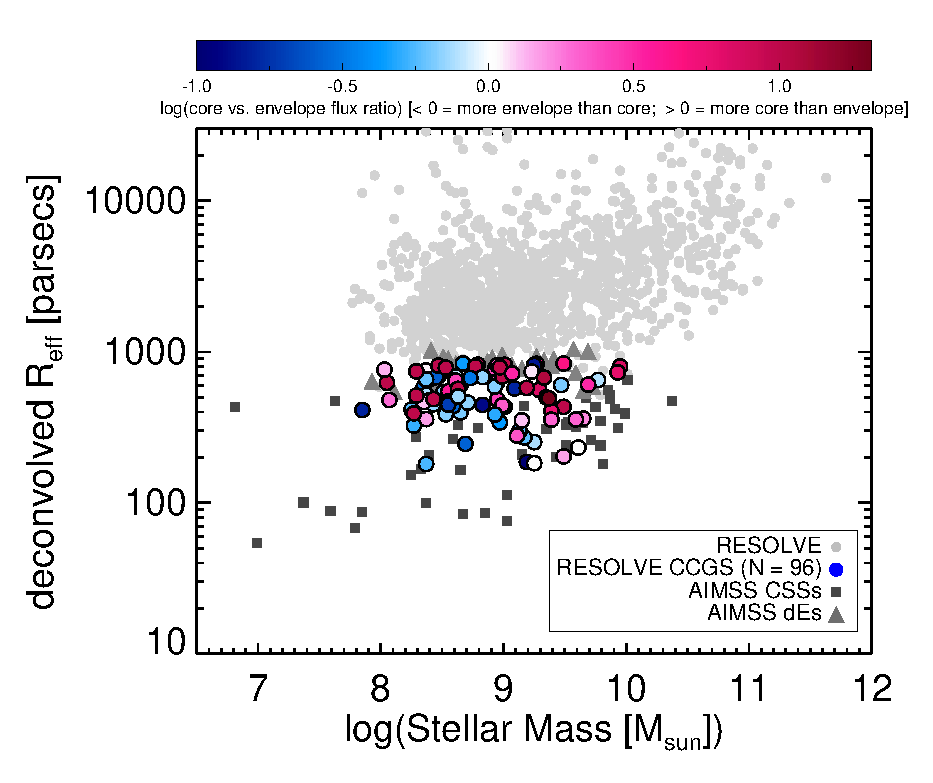
\includegraphics{Reff_Mstars.eps}
\caption{We plot here the deconvolved \Reff\ measurements for the entire RESOLVE sample, along with the CSSs of the AIMSS catalog. In grey are the RESOLVE (non-CCG) galaxies, which are plotted using their one component fit \Reff. The CCG sample is plotted using the core \Reff\ of the two component fits, which is why they may appear separated from the full RESOLVE sample. The colors of the CCGs represent the logarithm of the flux ratio between the core and envelope. Galaxies with log(flux ratio) near 0 will have both a core and envelope, while galaxies with log(flux ratio) $>~1$ will have more light in the core and log(flux ratio) $>~1$ will have more light in the envelope.}
\label{fig:radius}
\end{center}
\end{figure*}

We plot in \autoref{fig:radius} the deconvolved \Reff\ measurements for the entire RESOLVE sample, along with the CSSs and dEs of the AIMSS catalog. In grey are all RESOLVE galaxies, plotted using their one component fit \Reff. The CCG sample is plotted again with the core \Reff\ of the two component fits, causing them to shift down from the full RESOLVE sample. The symbol color for the CCGs represents the logarithm of the light ratio between the core and envelope, meaning that galaxies with log(flux ratio) near zero will have both a core and envelope, while galaxies with log(flux ratio) greater or less than zero will have more light in the core or envelope, respectively. We see in \autoref{fig:radius} that both core- and envelope-dominated CCGs tend to be at the higher end of the \Reff\ values, while core+envelope CCGs tend to be the lower \Reff\ values. There also are more core-dominated CCGs at the higher M$_{\star}$ end while envelope-dominated CCGs tend to reside at low M$_{\star}$.

\subsection{Colors and Star formation rates}

\begin{figure*}[hbpt!]
\begin{center}
\includegraphics[scale=0.65]{sfr_mbary.eps}
\caption{\textbf{(Left.)} On the left we plot the $u-r$ colors against stellar mass of CCGs with the entire RESOLVE sample. \textbf{(Right.)} On the right we have plotted the FSMGR against baryonic mass for both the CCGs and entire RESOLVE sample. }
\label{fig:fsmgr}
\end{center}
\end{figure*}

 We first examine the colors of the CCG sample. The left side of \autoref{fig:fsmgr} shows the k-corrected and extinction-corrected $u-r$ colors (as described in \autoref{phot}) of our CCG sample plotted against M$_{\star}$, compared to the RESOLVE sample as a whole. An unusual finding is that many CCGs live on the blue sequence, since most CSSs are most often thought of as being ``red and dead''. The right side of \autoref{fig:fsmgr} shows FSMGR vs. M$_{\rm bary}$ for the same objects. As with the colors, we find that many CCGs are forming stars at a rapid rate (FSMGR $\sim~1$ means that the galaxy has doubled its mass in the last Gyr), again an unexpected finding which could indicate that some CCGs are still in the process of forming (if dissipatively formed) or relaxing (if tidally-stripped remnants).

%add statistical test at some point

\begin{figure*}[hbpt!]
\begin{center}
\includegraphics{nn_groupmass_2d.eps}
\caption{We plot here the group halo mass against the nearest 3D neighbor for the RESOLVE survey and CCG sample. We see that CCGs live in a variety of environments, from extremely isolated (nearest neighbor $>$ 1 Mpc) to massive (M$_{\rm halo} \sim 10^{13}$ M$_{\odot}$) groups. There is no obvious trend into whether cores+envelopes and cores/envelopes preferentially live in different environments.}
\label{fig:envplot}
\end{center}
\end{figure*}

\subsection{Environments}
We investigate the distribution of CCGs throughout the cosmic web, and find that CCGs span a range of different environments (see \autoref{fig:envplot}). There are many CCGs residing in low mass groups, similar to the M32--Andromeda relationship, which suggests that tidal stripping could have occurred for those CCGs. On the opposite end, we see several CCGs in massive group halos, and these CCGs tend to be either core- or envelope dominated. This hints towards ram pressure stripping being at play in these environments, especially for those CCGs at larger distances from other galaxies. There are also nine CCGs that are $>1$ Mpc away from another object in RA--Dec--redshift space, and four of those are core dominated, resembling the isolated cE found by \citet{Huxor2013}. These free floating CCGs may be the result of dissipative formation since there is no nearby object to have performed the stripping or may have been ejected from groups or clusters during the stripping process.
 
 \begin{figure*}[b]
\begin{center}
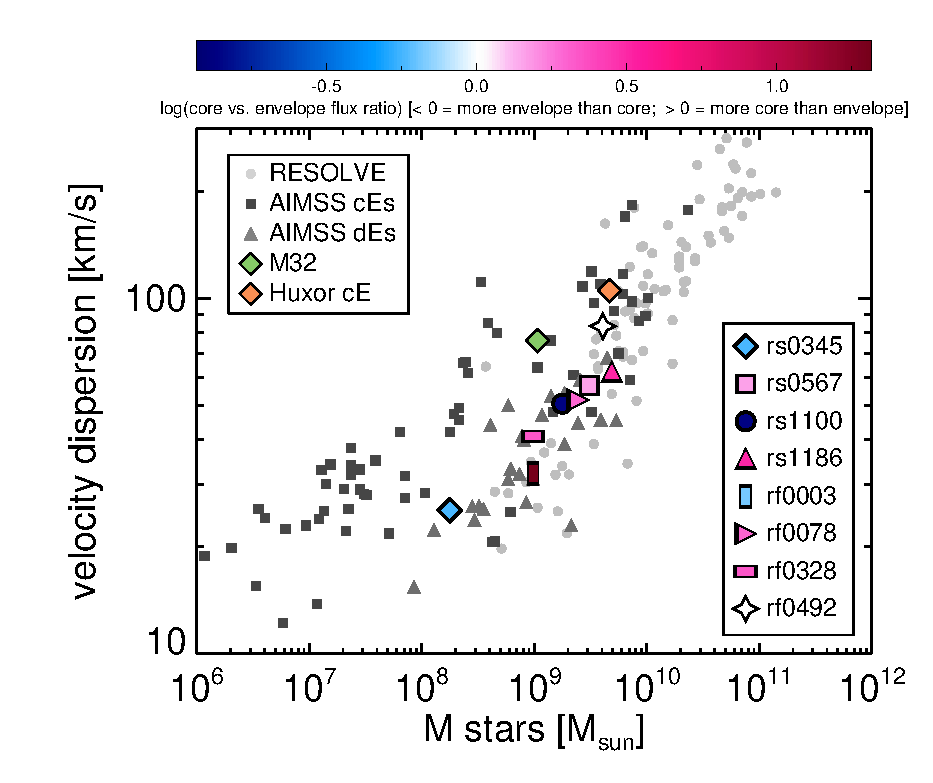
\includegraphics{faber-jackson_resolvesigmas.eps}
\caption{The Faber-Jackson relation (stellar mass vs. velocity dispersion) for the RESOLVE sample, CCGs, and the cEs and dEs of the AIMSS catalog. We look for CCGs offset to higher $\sigma$ for its stellar mass, which may indicate tidal stripping as a possible formation scenario. The green point is M32, the prototypical cE, that is believed to be tidally stripped \citep{Faber1973}. In orange is the free floating cE discovered in \citet{Huxor2013} that is thought to be dissipatively formed.}
\label{fig:sigma}
\end{center}
\end{figure*}
 
\subsection{Kinematics}
\label{kin}
 We lastly investigate the kinematics of the CCG sample using $\sigma$ values derived from SOAR and Gemini telescope data. \autoref{fig:sigma} plots the Faber-Jackson ($\sigma$-M$_{\star}$) relation for the 8 CCGs with $\sigma$ measurements along with the other 80+ RESOLVE galaxies with $\sigma$ measured. Galaxies with $\sigma$ offset to higher values point to tidal stripping occurring, since they will have less stellar mass than the motions of the stars suggest should be there. Conversely, galaxies with $\sigma$ that lie on the trend may point dissipative formation occurring, since these will have formed similarly to normal elliptical galaxies. Most CCGs seem to be following the dissipative merger track, and in \autoref{discussion}, we examine in depth the formation scenarios for each of these 8 CCGs with velocity dispersion measurements.

%%%%%%%%%%%%%%%%%%%%%%%%%%%%%%%
%%%%%%%%%%%%%%%%%%%%%%%%%%%%%%%
\section{CCG formation processes} %kind of like a discussion section
\label{discussion}

We now take an in depth look at the 8 CCGs with kinematics, and assign formation scenarios based on their core \Reff\, morphology, star formation histories, kinematics, and environments. For this discussion, we classify CCGs using the terms ``CSS-like'', ``dE-like'', or ``crossover''.  A CSS-like CCG will have a small core radius and a $\sigma$ value offset from the main Faber-Jackson relation, as expected for UCDs and cEs that have been tidally stripped. A dE-like CCG will have a large core radius and low $\sigma$ as is expected for dEs that are dissipatively formed. Crossover CCGs will have either large core radius and high $\sigma$ or small core radius and low $\sigma$. Following this logic, we classify M32 as CCS-like since it has \Reff~$\sim~100$~pc and $\sigma$ offset to higher dispersion. The cE discovered in \citet{Huxor2013} is a crossover, since it has \Reff~$\sim~500$~pc and a $\sigma$ value falling along the main Faber-Jackson relation.

We have replotted Figures 4, 5, and 6 in \autoref{fig:miniplots}, this time highlighting the eight CCGs with velocity dispersions only. An important caveat for the CSSs and dEs in the AIMSS catalog is that the radius measurements are not decomposed into one and two components. To correct for this, we plot in the top left panel of \autoref{fig:miniplots} the one component \Reff\ instead of the two component core \Reff\ so that we may accurately compare the radius measurements of CCGs to those of the AIMSS objects.

\subsection{dE-like CCGs}
We classify rs0345, rs1100, rf0003, and rf0328 as dE-like CCGs, based on their high one-component effective radius and low $\sigma$. The CCGs rs0345 and rs1100 are both envelope-dominated, live firmly on the blue sequence, and are forming stars quite rapidly with FSMGR~$>1$. The galaxies reside in intermediate-sized groups (halo masses $\sim10^{11.7-12.5}$~\Msun) and are both within $<~0.15$~Mpc from a companion galaxy. Taken together these data suggest that rs0345 and rs1100 may be an example of tidal stripping or dissipative processes actively occurring, which is fueling the star formation and funneling gas from the disk to build a core. Judging from the regular morphologies seen in the images of these CCGs in \autoref{fig:imageplots}, tidal stripping and dissipative formation via merging are unlikely, which leaves ram pressure stripping as a probable formation scenario.

CCG rf0003 is core-dominated, lives intermediate between the blue and red sequences and has a low FSMGR ($\sim~0.10$). It resides in a low mass group (halo mass $\sim10^{10.9}$~\Msun) and is $>2$~Mpc from another galaxy, which we classify as free floating. Its $\sigma$ places it firmly along the main Faber-Jackson relation. All together, these clues point to a dissipatively-formed CCG, perhaps through the convergence of cold streams. Residing near the green valley indicate that this formation may have occurred relatively recently.

Lastly, rf0328 is also core-dominated and lives intermediate between the blue and red sequences, but has a higher FSMGR at $\sim0.6$, indicating considerable star formation taking place in the last Gyr. The galaxy resides in a low mass group and is $\sim0.4$~Mpc from a neighbor. Its $\sigma$ places it among the dissipatively-formed CCGs, perhaps due to cold gas streams converging or even a merger, given its environment. Like rf0003, its color and FSMGR may indicate this formation happened recently.

\subsection{CSS-like CCGs}
We do not find any CSS-like CCGs in our subset of CCGs with kinematic data, however we expect that with additional velocity dispersion data, we will find CCGs following this track in the future.

\subsection{Crossover CCGs}
We classify rs0567, rs1186, rf0078, rf0492 as crossover CCGs, based on their small one component \Reff\ measurements ($\sim~500-700$~pc) and $\sigma$ values following the dissipative formation track. The CCGs rs0567, rs1186, and rf0078 are all three are mildly core-dominated galaxies. They live on the red sequence and display little star formation (FSMGR $> 0.1$) for all. CCGs rs1186 and rf0078 both have close neighbors ($\sim~0.2$~Mpc distance), but rs0567 has a nearest neighbor $\sim~0.7$~Mpc, which makes it quite similar to the free floating cE discovered by \citet{Huxor2013} (which also has a core-dominated light profile).

CCG rf0492 lies closest to the free floating cE from \citet{Huxor2013} in both \autoref{fig:sigma} and the top left of \autoref{fig:imageplots}, but they don't share many other similarities. This CCG has a core+envelope profile and lives in an intermediate-sized group with halo mass~$\sim~10^{12}$~\Msun and neighbor within $\sim~0.11$~Mpc. It lives on the red sequence and has low FSMGR ($<~0.1$), making it a good candidate of a CCG formed via ram pressure stripping as a dwarf (perhaps an LCBD) fell into the group halo.  

We note that there are two cEs in AIMSS with extremely small \Reff\ and low $\sigma$ (the dark squares at M$_{\star}~\sim~10^{8.5}$~\Msun\ and $\sigma~\sim~20~\text{km~s}^{-2}$ in \autoref{fig:sigma}), and we classify these as crossovers as well. We postulate that galaxies like these and the other crossover CCGs discussed above may be the low-$z$ analogues to the ``red/blue nugget'' galaxies that are common at high-redshift with \Reff~$<~1$~kpc. \citet{Dekel2013} propose that at high redshifts, blue nuggets form when gaseous disks contract during dissipative processes (such as gas inflows to the central region of the disk) and then later quench to become red nuggets that are so common in the early Universe.

There are also two AIMSS objects with the opposite conditions: large \Reff\ and high $\sigma$ (the two dark triangles in \autoref{fig:sigma} with M$_{\star}~\sim~10^{8.5}$~\Msun\ and $\sigma~\sim~40-50~\text{km~s}^{-2}$). These dEs may be in the process of tidal stripping currently and may move to the CSS-like track when the stripping is complete.

\begin{figure*}[b]
\begin{center}
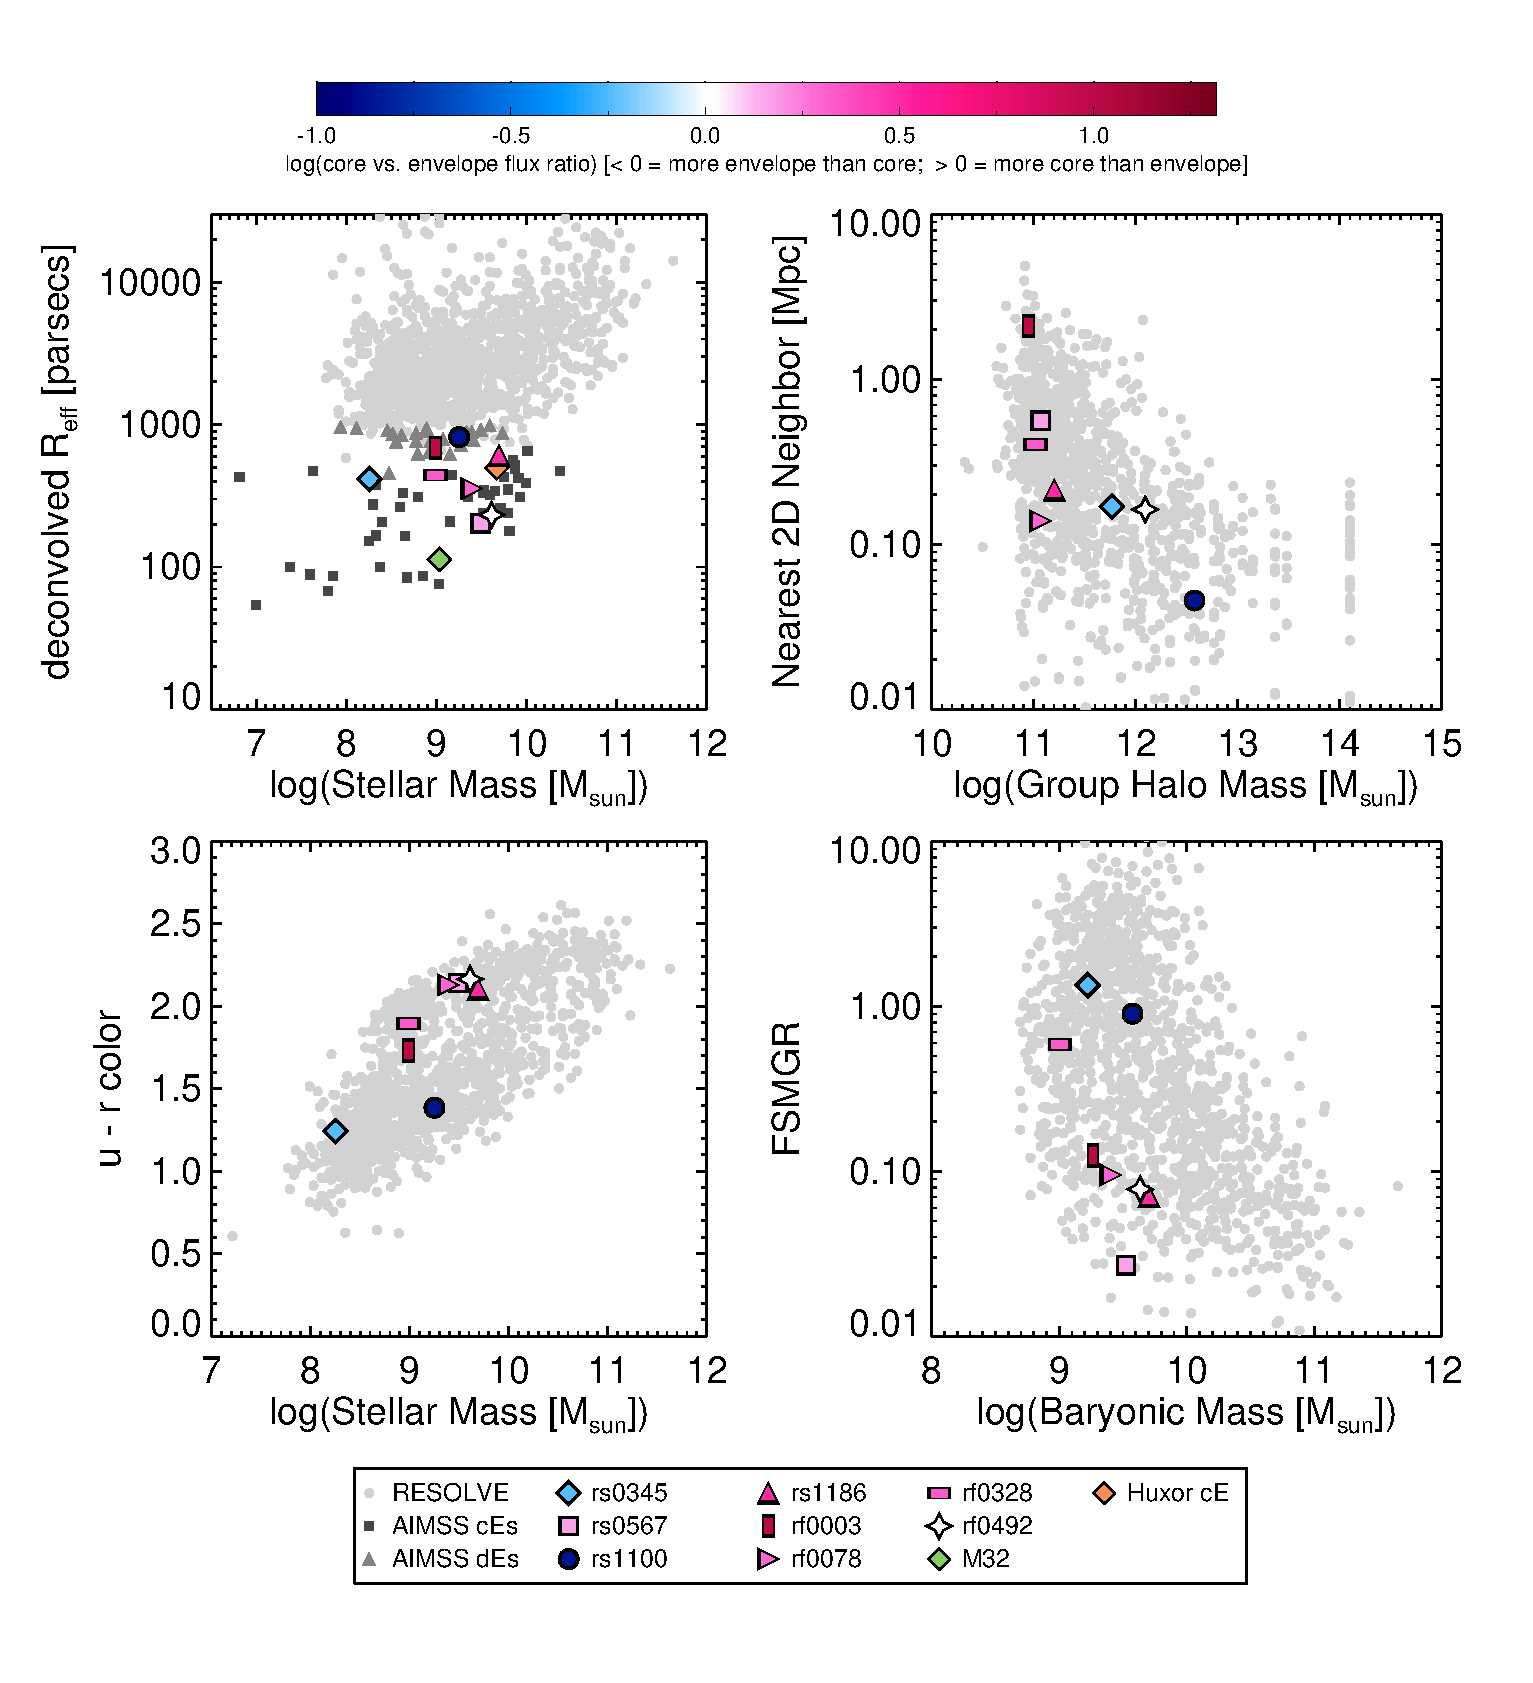
\includegraphics[scale=0.7]{miniplots.eps}
\caption{\textbf{(Top left.)} single-component deconvolved \Reff\ vs. stellar mass, \textbf{(Top right.)} the nearest two-dimensional neighbor vs. group halo mass, \textbf{(Bottom left.)} $u-r$ color vs. stellar mass, and \textbf{(Bottom right.)} FSMGR vs. baryonic mass for all galaxies in RESOLVE, the cEs and dEs of AIMSS, and the eight CCGs that have velocity dispersion information. We emphasize that the \Reff\ values plotted in the top left panel are not the two-component core \Reff\ values as in \autoref{fig:radius} in order to compare our radius measurements with the CSSs of AIMSS that have not been decomposed.}
\label{fig:miniplots}
\end{center}
\end{figure*}

\begin{figure*}[b]
\begin{center}
\includegraphics[scale=0.7]{imageplots.eps}
\caption{The light profiles for the eight CCGs with velocity dipersion measurements. The $rgb$ images are from the SDSS-DR8 image list tool. Above each plot is the value of the logarithm of the ratio of the core and envelope fluxes, which are given via the symbol colors in \autoref{fig:sigma} and \autoref{fig:miniplots}. We also note that rf0003 is one of the six cases where \textsc{Galfit} finds identical \Reff\ values for both the first and second S\'ersic components, and have hence set log(flux ratio) = maximum of all flux ratios ($+1.31$).}
\label{fig:imageplots}
\end{center}
\end{figure*}

%\subsection{CCGs without velocity dispersions}

%For the other 88 CCGs without velocity dispersions, we attempt to classify their formation scenarios using the above cases as a primer. We divide the above 8 CCGs into four categories: ``forming with uncertain origins'' (rs0345, rs1100), ``recently formed with dissipative origins likely'' (rf0003, rf0328), ``uncertain stripping and dissipative formation'' (rf0492), and ``likely dissipatively formed'' (rs0567, rs1186, rf0078).

%``Forming with uncertain origins'' CCGs are easily characterized as having envelopes (log(flux ratio) $<$ -0.1), high FSMGR ($>0.5$), and living in high mass groups ($>10^{11.5}$~\Msun). There are 6 CCGs with these parameters ($\sim1\%$ of the sample), including the two already identified. CCGs in the ``likely dissipatively formed'' are also easy characterized by having cores (log(flux ratio) $>$ 0.1), low FSMGR ($>0.5$), and living in low mass groups ($>10^{11.5}$~\Msun). There are 21 CCGs with these parameters ($\sim21\%$ of the sample), again including the three already identified. This leaves 66 CCGs left to classify, but the remaining groups, ``uncertain stripping and dissipative formation'' and ``recently formed'' are more difficult to classify definitely due to their ranges of colors, morphologies, and environments. This leaves $\sim69\%$ of the CCG unclassified until more velocity information is available.

%%%%%%%%%%%%%%%%%%%%%%%%%%%%%%%
%%%%%%%%%%%%%%%%%%%%%%%%%%%%%%%
\section{Conclusions}
\label{conclusions}

  In this paper we have examined the colors, FSMGR, environments, and kinematics of the 96 compact core galaxies (CCGs) in the RESOLVE survey. We have selected CCGs to have a seeing-deconvolved, core-only \Reff\ $<$ 800 pc, based on the sizes of the compact and dwarf ellipticals in the AIMSS catalog. We have quantified the amount of light in the cores and envelopes of each CCG by performing two component fits with \textsc{Galfit} and taking the logarithm of the ratio of the fluxes of the two different components. CCGs with more light in the envelope have log(flux ratio) $<$ 0 and are called ``envelope-dominated' CCGs. CCGs with more light in the core have log(flux ratio) $>$ 0 and are called ``core-dominated'' CCGs. CCGs with log(flux ratio) $\sim 0$ have both a bright core plus an extended envelope and are called ``core+envelope'' CCGs. Our main results can be summarized as follows:

\begin{enumerate}
\item \autoref{fig:radius} shows that both core- and envelope-dominated CCGs tend to be at the higher end of the \Reff\ values, while core+envelope CCGs tend to be the lower \Reff\ values. There also are more core-dominated CCGs at the higher M$_{\star}$ end while envelope-dominated CCGs tend to reside at low M$_{\star}$.

\item We find that many CCGs live on the blue sequence and are forming stars at a rapid rate (see \autoref{fig:fsmgr}), which could indicate that some CCGs are still in the process of forming (if dissipatively formed) or relaxing (if a tidally-stripped remnant).

\item We find that CCGs span a range of different environments (see \autoref{fig:envplot}). Many CCGs live in low mass groups, similar to the M32--Andromeda relationship, perhaps hinting at tidal stripping formation scenarios. Others live in massive group halos and tend to be either core- or envelope dominated CCGs, conversely hinting towards ram pressure stripping being at play. There are also many CCGs that are $>1$ Mpc away from another object in RA--Dec--redshift space, resembling the isolated cEs found by \citet{Huxor2013} and \citet{Paudel2014}, which may point to a dissipative formation scenario.

\item Using velocity dispersions ($\sigma$) derived from the SOAR and Gemini telescopes, we classify the eight CCGs with $\sigma$ measurements as ``CCS-like'', ``dE-like'', or ``crossover'', based on their one-component radius measurements (the top left panel of \autoref{fig:miniplots}) and position on the Faber-Jackson ($\sigma$-M$_{\star}$) relation (\autoref{fig:sigma}). We find four CCGs that are dE-like and four that are crossovers.

%In \autoref{fig:sigma}, we find that 6 CCGs tend to follow the main Faber-Jackson trend, which is expected for galaxies formed via dissipative formation, and two CCGs that may be slightly offset to higher $\sigma$. 

%\item Using the 8 CCGs with velocity dispersions as a primer, we attempt to quantify the number of CCGs that are tidally stripped or dissipatively formed based on morphologies, colors, FSMGR, and environment. We estimate $\sim$6\% of CCGs are actively forming (though the driver is uncertain) and $\sim$21\% are likely dissipatively formed. The remaining $\sim69$\% need more information to be classified.
\end{enumerate}

  Future work will include the following:

\begin{enumerate}

\item \textit{Redefine CCG sample using $\chi^2$ analysis.} As mentioned in \autoref{CCGs}, we want to redefine the CCG sample using the $\chi^2$ and number of degrees of freedom (NoDF) output by \textsc{Galfit} for each fit. This will entail using the $\chi^2$ and NoDF to decide whether the one or two component fits are best for all RESOLVE galaxies. Those best fit with one component would then be selected as a CCG if its one component \Reff\ is less than 800~pc, while those best fit with two components would be selected as a CCG if its core \Reff\ is less than 800~pc. This method replace the arbitrary cutoff for CCG candidates at \Reff~$<~1$~kpc, which should let us include more CCGs that have large diffuse envelopes and small cores that may be getting left out of our sample now.

\item \textit{Investigate gas content.} The amount of neutral Hydrogen gas CCGs have may give us insights into their evolution over time. For example, a CCG in a galaxy cluster with little HI gas may point towards ram pressure stripping being important. Combined with CCG colors and FSMGR, the gas content may be an important tool in determining the evolution of a CCG.

\item \textit{Investigate metallicities.} \citet{Janz2015} have shown that tidally-stripped CSSs are systematically offset to higher metal abundances. With the SOAR and Gemini spectroscopy currently in hand, we will be able to test this hypothesis for the CCG sample and use this method as another way to discern formation scenarios.

\end{enumerate}

  \acknowledgments{ \textit{Acknowledgments.}
This work has been supported by funding from NSF grants AST-0955368 and OCI-1156614 and NASA grant HST-AR-12147.01-A. 
This work is based on data obtained as part of the UKIRT Infrared Deep Sky Survey. This work is based on observations obtained at the Gemini Observatory under program numbers GS-2013B-Q52, GS-2014B-Q-13, GS-2014B-Q-51, and GS-2015B-C-1, which is operated by the Association of Universities for Research in Astronomy, Inc., under a cooperative agreement with the NSF on behalf of the Gemini partnership: the National Science Foundation (United States), the National Research Council (Canada), CONICYT (Chile), Ministerio de Ciencia, Tecnolog\'{i}a e Innovaci\'{o}n Productiva (Argentina), and Minist\'{e}rio da Ci\^{e}ncia, Tecnologia e Inova\c{c}\~{a}o (Brazil).}

\bibliographystyle{apj}
\bibliography{library.bib}

\appendix
\label{app}

\end{document}
              
